\documentclass[convert = false, tikz]{standalone}
\usepackage[utf8]{inputenc}
\usepackage{tikz}
\usetikzlibrary{automata, positioning, arrows, shapes.geometric, decorations.pathmorphing}

\usepackage{../../../../style_automata}

% arara: pdflatex
% arara: latexmk: { clean: partial }
\begin{document}
    \tikzset{
    node distance=2cm, % specifies the minimum distance between two nodes.
    }

    \scalebox{0.8}{
    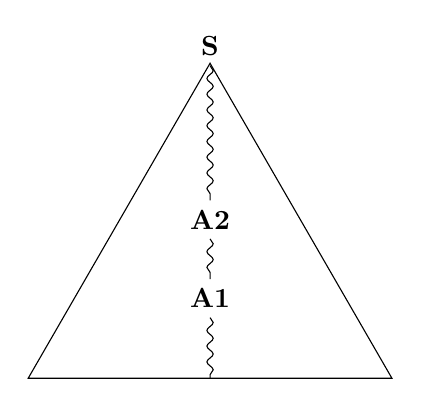
\begin{tikzpicture}

    % Apex angle 60 degrees
    \node[isosceles triangle, rotate=90, isosceles triangle apex angle=60, draw, minimum size=4cm] (T) {};
    \draw[] ([yshift=0.2cm]T.apex) node[](S){\textbf{S}};
    \draw[] ([yshift=-2cm]T.apex) node[](A2){\textbf{A2}};
    \draw[] ([yshift=-3cm]T.apex) node[](A1){\textbf{A1}};

    \draw [decorate,decoration={snake,amplitude=.4mm,segment length=2mm,post length=0mm}] (S.south) -- (A2.north);
    \draw [decorate,decoration={snake,amplitude=.4mm,segment length=2mm,post length=0mm}] (A2.south) -- (A1.north);
    \draw [decorate,decoration={snake,amplitude=.4mm,segment length=2mm,post length=0mm}] (A1.south) -- (T.lower side);
    
    \end{tikzpicture}
    }
\end{document}